\documentclass[1p]{elsarticle_modified}
%\bibliographystyle{elsarticle-num}

%\usepackage[colorlinks]{hyperref}
%\usepackage{abbrmath_seonhwa} %\Abb, \Ascr, \Acal ,\Abf, \Afrak
\usepackage{amsfonts}
\usepackage{amssymb}
\usepackage{amsmath}
\usepackage{amsthm}
\usepackage{scalefnt}
\usepackage{amsbsy}
\usepackage{kotex}
\usepackage{caption}
\usepackage{subfig}
\usepackage{color}
\usepackage{graphicx}
\usepackage{xcolor} %% white, black, red, green, blue, cyan, magenta, yellow
\usepackage{float}
\usepackage{setspace}
\usepackage{hyperref}

\usepackage{tikz}
\usetikzlibrary{arrows}

\usepackage{multirow}
\usepackage{array} % fixed length table
\usepackage{hhline}

%%%%%%%%%%%%%%%%%%%%%
\makeatletter
\renewcommand*\env@matrix[1][\arraystretch]{%
	\edef\arraystretch{#1}%
	\hskip -\arraycolsep
	\let\@ifnextchar\new@ifnextchar
	\array{*\c@MaxMatrixCols c}}
\makeatother %https://tex.stackexchange.com/questions/14071/how-can-i-increase-the-line-spacing-in-a-matrix
%%%%%%%%%%%%%%%

\usepackage[normalem]{ulem}

\newcommand{\msout}[1]{\ifmmode\text{\sout{\ensuremath{#1}}}\else\sout{#1}\fi}
%SOURCE: \msout is \stkout macro in https://tex.stackexchange.com/questions/20609/strikeout-in-math-mode

\newcommand{\cancel}[1]{
	\ifmmode
	{\color{red}\msout{#1}}
	\else
	{\color{red}\sout{#1}}
	\fi
}

\newcommand{\add}[1]{
	{\color{blue}\uwave{#1}}
}

\newcommand{\replace}[2]{
	\ifmmode
	{\color{red}\msout{#1}}{\color{blue}\uwave{#2}}
	\else
	{\color{red}\sout{#1}}{\color{blue}\uwave{#2}}
	\fi
}

\newcommand{\Sol}{\mathcal{S}} %segment
\newcommand{\D}{D} %diagram
\newcommand{\A}{\mathcal{A}} %arc


%%%%%%%%%%%%%%%%%%%%%%%%%%%%%5 test

\def\sl{\operatorname{\textup{SL}}(2,\Cbb)}
\def\psl{\operatorname{\textup{PSL}}(2,\Cbb)}
\def\quan{\mkern 1mu \triangleright \mkern 1mu}

\theoremstyle{definition}
\newtheorem{thm}{Theorem}[section]
\newtheorem{prop}[thm]{Proposition}
\newtheorem{lem}[thm]{Lemma}
\newtheorem{ques}[thm]{Question}
\newtheorem{cor}[thm]{Corollary}
\newtheorem{defn}[thm]{Definition}
\newtheorem{exam}[thm]{Example}
\newtheorem{rmk}[thm]{Remark}
\newtheorem{alg}[thm]{Algorithm}

\newcommand{\I}{\sqrt{-1}}
\begin{document}

%\begin{frontmatter}
%
%\title{Boundary parabolic representations of knots up to 8 crossings}
%
%%% Group authors per affiliation:
%\author{Yunhi Cho} 
%\address{Department of Mathematics, University of Seoul, Seoul, Korea}
%\ead{yhcho@uos.ac.kr}
%
%
%\author{Seonhwa Kim} %\fnref{s_kim}}
%\address{Center for Geometry and Physics, Institute for Basic Science, Pohang, 37673, Korea}
%\ead{ryeona17@ibs.re.kr}
%
%\author{Hyuk Kim}
%\address{Department of Mathematical Sciences, Seoul National University, Seoul 08826, Korea}
%\ead{hyukkim@snu.ac.kr}
%
%\author{Seokbeom Yoon}
%\address{Department of Mathematical Sciences, Seoul National University, Seoul, 08826,  Korea}
%\ead{sbyoon15@snu.ac.kr}
%
%\begin{abstract}
%We find all boundary parabolic representation of knots up to 8 crossings.
%
%\end{abstract}
%\begin{keyword}
%    \MSC[2010] 57M25 
%\end{keyword}
%
%\end{frontmatter}

%\linenumbers
%\tableofcontents
%
\newcommand\colored[1]{\textcolor{white}{\rule[-0.35ex]{0.8em}{1.4ex}}\kern-0.8em\color{red} #1}%
%\newcommand\colored[1]{\textcolor{white}{ #1}\kern-2.17ex	\textcolor{white}{ #1}\kern-1.81ex	\textcolor{white}{ #1}\kern-2.15ex\color{red}#1	}

{\Large $\underline{10_{106}~(K10a_{95})}$}

\setlength{\tabcolsep}{10pt}
\renewcommand{\arraystretch}{1.6}
\vspace{1cm}\begin{tabular}{m{100pt}>{\centering\arraybackslash}m{274pt}}
\multirow{5}{120pt}{
	\centering
	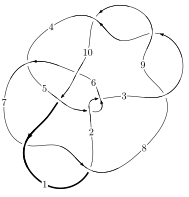
\includegraphics[width=112pt]{../../../GIT/diagram.site/Diagrams/png/190_10_106.png}\\
\ \ \ A knot diagram\footnotemark}&
\allowdisplaybreaks
\textbf{Linearized knot diagam} \\
\cline{2-2}
 &
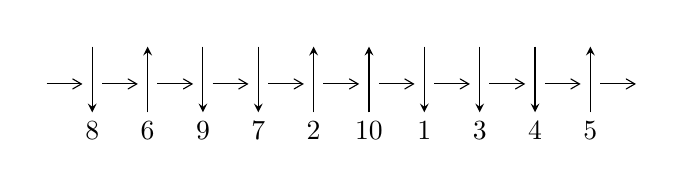
\begin{tikzpicture}[x=20pt, y=17pt]
	% nodes
	\node (C0) at (0, 0) {};
	\node (C1) at (1, 0) {};
	\node (C1U) at (1, +1) {};
	\node (C1D) at (1, -1) {8};

	\node (C2) at (2, 0) {};
	\node (C2U) at (2, +1) {};
	\node (C2D) at (2, -1) {6};

	\node (C3) at (3, 0) {};
	\node (C3U) at (3, +1) {};
	\node (C3D) at (3, -1) {9};

	\node (C4) at (4, 0) {};
	\node (C4U) at (4, +1) {};
	\node (C4D) at (4, -1) {7};

	\node (C5) at (5, 0) {};
	\node (C5U) at (5, +1) {};
	\node (C5D) at (5, -1) {2};

	\node (C6) at (6, 0) {};
	\node (C6U) at (6, +1) {};
	\node (C6D) at (6, -1) {10};

	\node (C7) at (7, 0) {};
	\node (C7U) at (7, +1) {};
	\node (C7D) at (7, -1) {1};

	\node (C8) at (8, 0) {};
	\node (C8U) at (8, +1) {};
	\node (C8D) at (8, -1) {3};

	\node (C9) at (9, 0) {};
	\node (C9U) at (9, +1) {};
	\node (C9D) at (9, -1) {4};

	\node (C10) at (10, 0) {};
	\node (C10U) at (10, +1) {};
	\node (C10D) at (10, -1) {5};
	\node (C11) at (11, 0) {};

	% arrows
	\draw[->,>={angle 60}]
	(C0) edge (C1) (C1) edge (C2) (C2) edge (C3) (C3) edge (C4) (C4) edge (C5) (C5) edge (C6) (C6) edge (C7) (C7) edge (C8) (C8) edge (C9) (C9) edge (C10) (C10) edge (C11) ;	\draw[->,>=stealth]
	(C1U) edge (C1D) (C2D) edge (C2U) (C3U) edge (C3D) (C4U) edge (C4D) (C5D) edge (C5U) (C6D) edge (C6U) (C7U) edge (C7D) (C8U) edge (C8D) (C9U) edge (C9D) (C10D) edge (C10U) ;
	\end{tikzpicture} \\
\hhline{~~} \\& 
\textbf{Solving Sequence} \\ \cline{2-2} 
 &
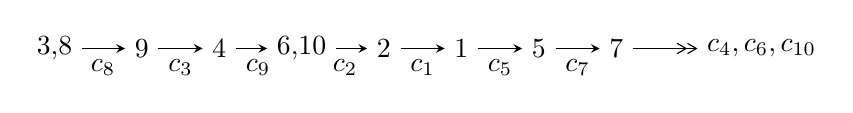
\begin{tikzpicture}[x=28pt, y=7pt]
	% node
	\node (A0) at (-1/8, 0) {3,8};
	\node (A1) at (1, 0) {9};
	\node (A2) at (2, 0) {4};
	\node (A3) at (49/16, 0) {6,10};
	\node (A4) at (33/8, 0) {2};
	\node (A5) at (41/8, 0) {1};
	\node (A6) at (49/8, 0) {5};
	\node (A7) at (57/8, 0) {7};
	\node (C1) at (1/2, -1) {$c_{8}$};
	\node (C2) at (3/2, -1) {$c_{3}$};
	\node (C3) at (5/2, -1) {$c_{9}$};
	\node (C4) at (29/8, -1) {$c_{2}$};
	\node (C5) at (37/8, -1) {$c_{1}$};
	\node (C6) at (45/8, -1) {$c_{5}$};
	\node (C7) at (53/8, -1) {$c_{7}$};
	\node (A8) at (9, 0) {$c_{4},c_{6},c_{10}$};

	% edge
	\draw[->,>=stealth]	
	(A0) edge (A1) (A1) edge (A2) (A2) edge (A3) (A3) edge (A4) (A4) edge (A5) (A5) edge (A6) (A6) edge (A7) ;
	\draw[->>,>={angle 60}]	
	(A7) edge (A8);
\end{tikzpicture} \\ 

\end{tabular} \\

\footnotetext{
The image of knot diagram is generated by the software ``\textbf{Draw programme}" developed by Andrew Bartholomew(\url{http://www.layer8.co.uk/maths/draw/index.htm\#Running-draw}), where we modified some parts for our purpose(\url{https://github.com/CATsTAILs/LinksPainter}).
}\phantom \\ \newline 
\centering \textbf{Ideals for irreducible components\footnotemark of $X_{\text{par}}$} 
 
\begin{align*}
I^u_{1}&=\langle 
-4.48988\times10^{22} u^{38}-3.35873\times10^{21} u^{37}+\cdots+1.23445\times10^{23} b-2.68996\times10^{23},\\
\phantom{I^u_{1}}&\phantom{= \langle  }7.60416\times10^{23} u^{38}-5.87608\times10^{23} u^{37}+\cdots+1.23445\times10^{23} a-3.17189\times10^{24},\;u^{39}- u^{38}+\cdots-12 u+1\rangle \\
I^u_{2}&=\langle 
u^4+u^3-2 u^2+b- u+1,\;u^6- u^5-4 u^4+4 u^3+3 u^2+a-3 u+1,\;u^7-4 u^5+u^4+4 u^3-2 u^2+1\rangle \\
I^u_{3}&=\langle 
u^3+b- u,\;a+u,\;u^4- u^3-1\rangle \\
I^u_{4}&=\langle 
b,\;a-1,\;u+1\rangle \\
\\
\end{align*}
\raggedright * 4 irreducible components of $\dim_{\mathbb{C}}=0$, with total 51 representations.\\
\footnotetext{All coefficients of polynomials are rational numbers. But the coefficients are sometimes approximated in decimal forms when there is not enough margin.}
\newpage
\renewcommand{\arraystretch}{1}
\centering \section*{I. $I^u_{1}= \langle -4.49\times10^{22} u^{38}-3.36\times10^{21} u^{37}+\cdots+1.23\times10^{23} b-2.69\times10^{23},\;7.60\times10^{23} u^{38}-5.88\times10^{23} u^{37}+\cdots+1.23\times10^{23} a-3.17\times10^{24},\;u^{39}- u^{38}+\cdots-12 u+1 \rangle$}
\flushleft \textbf{(i) Arc colorings}\\
\begin{tabular}{m{7pt} m{180pt} m{7pt} m{180pt} }
\flushright $a_{3}=$&$\begin{pmatrix}0\\u\end{pmatrix}$ \\
\flushright $a_{8}=$&$\begin{pmatrix}1\\0\end{pmatrix}$ \\
\flushright $a_{9}=$&$\begin{pmatrix}1\\u^2\end{pmatrix}$ \\
\flushright $a_{4}=$&$\begin{pmatrix}- u\\- u^3+u\end{pmatrix}$ \\
\flushright $a_{6}=$&$\begin{pmatrix}-6.15999 u^{38}+4.76010 u^{37}+\cdots-199.096 u+25.6949\\0.363717 u^{38}+0.0272084 u^{37}+\cdots-15.2996 u+2.17908\end{pmatrix}$ \\
\flushright $a_{10}=$&$\begin{pmatrix}- u^2+1\\- u^4+2 u^2\end{pmatrix}$ \\
\flushright $a_{2}=$&$\begin{pmatrix}6.10160 u^{38}-5.05142 u^{37}+\cdots+243.206 u-37.0950\\-1.08737 u^{38}+0.953945 u^{37}+\cdots-39.0834 u+4.92208\end{pmatrix}$ \\
\flushright $a_{1}=$&$\begin{pmatrix}5.01423 u^{38}-4.09747 u^{37}+\cdots+204.123 u-32.1729\\-1.08737 u^{38}+0.953945 u^{37}+\cdots-39.0834 u+4.92208\end{pmatrix}$ \\
\flushright $a_{5}=$&$\begin{pmatrix}3.85842 u^{38}-3.05742 u^{37}+\cdots+127.285 u-20.9953\\0.129593 u^{38}+0.0772817 u^{37}+\cdots-8.16390 u+2.14319\end{pmatrix}$ \\
\flushright $a_{7}=$&$\begin{pmatrix}-5.60239 u^{38}+4.54940 u^{37}+\cdots-197.298 u+25.4505\\0.341348 u^{38}+0.0105311 u^{37}+\cdots-12.5393 u+1.90327\end{pmatrix}$\\&\end{tabular}
\flushleft \textbf{(ii) Obstruction class $= -1$}\\~\\
\flushleft \textbf{(iii) Cusp Shapes $= -\frac{1385017988288929065913488}{123444509404697939971901} u^{38}+\frac{961354782874772297950502}{123444509404697939971901} u^{37}+\cdots-\frac{42223327798922175146355847}{123444509404697939971901} u+\frac{4715398000555894355706065}{123444509404697939971901}$}\\~\\
\newpage\renewcommand{\arraystretch}{1}
\flushleft \textbf{(iv) u-Polynomials at the component}\newline \\
\begin{tabular}{m{50pt}|m{274pt}}
Crossings & \hspace{64pt}u-Polynomials at each crossing \\
\hline $$\begin{aligned}c_{1},c_{7}\end{aligned}$$&$\begin{aligned}
&u^{39}-5 u^{38}+\cdots-30 u+4
\end{aligned}$\\
\hline $$\begin{aligned}c_{2},c_{5}\end{aligned}$$&$\begin{aligned}
&u^{39}-2 u^{38}+\cdots-3 u+1
\end{aligned}$\\
\hline $$\begin{aligned}c_{3},c_{8},c_{9}\end{aligned}$$&$\begin{aligned}
&u^{39}- u^{38}+\cdots-12 u+1
\end{aligned}$\\
\hline $$\begin{aligned}c_{4}\end{aligned}$$&$\begin{aligned}
&u^{39}-3 u^{38}+\cdots+145 u-47
\end{aligned}$\\
\hline $$\begin{aligned}c_{6}\end{aligned}$$&$\begin{aligned}
&u^{39}-3 u^{38}+\cdots-10 u-19
\end{aligned}$\\
\hline $$\begin{aligned}c_{10}\end{aligned}$$&$\begin{aligned}
&u^{39}+u^{38}+\cdots+6 u+1
\end{aligned}$\\
\hline
\end{tabular}\\~\\
\newpage\renewcommand{\arraystretch}{1}
\flushleft \textbf{(v) Riley Polynomials at the component}\newline \\
\begin{tabular}{m{50pt}|m{274pt}}
Crossings & \hspace{64pt}Riley Polynomials at each crossing \\
\hline $$\begin{aligned}c_{1},c_{7}\end{aligned}$$&$\begin{aligned}
&y^{39}-27 y^{38}+\cdots+44 y-16
\end{aligned}$\\
\hline $$\begin{aligned}c_{2},c_{5}\end{aligned}$$&$\begin{aligned}
&y^{39}-18 y^{38}+\cdots+9 y-1
\end{aligned}$\\
\hline $$\begin{aligned}c_{3},c_{8},c_{9}\end{aligned}$$&$\begin{aligned}
&y^{39}-43 y^{38}+\cdots+34 y-1
\end{aligned}$\\
\hline $$\begin{aligned}c_{4}\end{aligned}$$&$\begin{aligned}
&y^{39}-11 y^{38}+\cdots+39261 y-2209
\end{aligned}$\\
\hline $$\begin{aligned}c_{6}\end{aligned}$$&$\begin{aligned}
&y^{39}+9 y^{38}+\cdots-4118 y-361
\end{aligned}$\\
\hline $$\begin{aligned}c_{10}\end{aligned}$$&$\begin{aligned}
&y^{39}+y^{38}+\cdots+76 y-1
\end{aligned}$\\
\hline
\end{tabular}\\~\\
\newpage\flushleft \textbf{(vi) Complex Volumes and Cusp Shapes}
$$\begin{array}{c|c|c}  
\text{Solutions to }I^u_{1}& \I (\text{vol} + \sqrt{-1}CS) & \text{Cusp shape}\\
 \hline 
\begin{aligned}
u &= -0.526234 + 0.893865 I \\
a &= \phantom{-}0.080741 + 1.260370 I \\
b &= \phantom{-}0.77528 - 1.59615 I\end{aligned}
 & -0.67462 + 9.52466 I & -2.84539 - 8.01548 I \\ \hline\begin{aligned}
u &= -0.526234 - 0.893865 I \\
a &= \phantom{-}0.080741 - 1.260370 I \\
b &= \phantom{-}0.77528 + 1.59615 I\end{aligned}
 & -0.67462 - 9.52466 I & -2.84539 + 8.01548 I \\ \hline\begin{aligned}
u &= -0.891332\phantom{ +0.000000I} \\
a &= \phantom{-}0.948472\phantom{ +0.000000I} \\
b &= -0.173901\phantom{ +0.000000I}\end{aligned}
 & -1.64188\phantom{ +0.000000I} & -6.13450\phantom{ +0.000000I} \\ \hline\begin{aligned}
u &= -0.753681 + 0.913845 I \\
a &= -0.775515 - 0.367156 I \\
b &= -0.034229 + 1.332130 I\end{aligned}
 & -1.18856 - 3.53262 I & \phantom{-0.000000 -}0. + 6.78010 I \\ \hline\begin{aligned}
u &= -0.753681 - 0.913845 I \\
a &= -0.775515 + 0.367156 I \\
b &= -0.034229 - 1.332130 I\end{aligned}
 & -1.18856 + 3.53262 I & \phantom{-0.000000 } 0. - 6.78010 I \\ \hline\begin{aligned}
u &= \phantom{-}0.449207 + 0.638779 I \\
a &= -0.54432 + 1.40207 I \\
b &= \phantom{-}0.02023 - 1.45003 I\end{aligned}
 & \phantom{-}3.29761 - 4.06547 I & \phantom{-}1.75322 + 6.53958 I \\ \hline\begin{aligned}
u &= \phantom{-}0.449207 - 0.638779 I \\
a &= -0.54432 - 1.40207 I \\
b &= \phantom{-}0.02023 + 1.45003 I\end{aligned}
 & \phantom{-}3.29761 + 4.06547 I & \phantom{-}1.75322 - 6.53958 I \\ \hline\begin{aligned}
u &= \phantom{-}0.587174 + 0.474790 I \\
a &= -0.976192 - 0.745918 I \\
b &= -0.028896 - 0.602541 I\end{aligned}
 & -3.42290 - 4.16688 I & -6.75958 + 5.97205 I \\ \hline\begin{aligned}
u &= \phantom{-}0.587174 - 0.474790 I \\
a &= -0.976192 + 0.745918 I \\
b &= -0.028896 + 0.602541 I\end{aligned}
 & -3.42290 + 4.16688 I & -6.75958 - 5.97205 I \\ \hline\begin{aligned}
u &= \phantom{-}0.556467 + 0.391333 I \\
a &= \phantom{-}1.46828 - 1.00646 I \\
b &= \phantom{-}0.434310 + 0.698478 I\end{aligned}
 & \phantom{-}2.85501 + 0.22937 I & \phantom{-}3.06420 + 0.82307 I\\
 \hline 
 \end{array}$$\newpage$$\begin{array}{c|c|c}  
\text{Solutions to }I^u_{1}& \I (\text{vol} + \sqrt{-1}CS) & \text{Cusp shape}\\
 \hline 
\begin{aligned}
u &= \phantom{-}0.556467 - 0.391333 I \\
a &= \phantom{-}1.46828 + 1.00646 I \\
b &= \phantom{-}0.434310 - 0.698478 I\end{aligned}
 & \phantom{-}2.85501 - 0.22937 I & \phantom{-}3.06420 - 0.82307 I \\ \hline\begin{aligned}
u &= \phantom{-}1.345600 + 0.177030 I \\
a &= -0.659060 + 0.853206 I \\
b &= -0.77984 - 1.42084 I\end{aligned}
 & -3.63229 - 5.60644 I & \phantom{-0.000000 } 0 \\ \hline\begin{aligned}
u &= \phantom{-}1.345600 - 0.177030 I \\
a &= -0.659060 - 0.853206 I \\
b &= -0.77984 + 1.42084 I\end{aligned}
 & -3.63229 + 5.60644 I & \phantom{-0.000000 } 0 \\ \hline\begin{aligned}
u &= \phantom{-}1.357030 + 0.066004 I \\
a &= \phantom{-}0.377431 + 0.276144 I \\
b &= \phantom{-}0.13369 - 1.70062 I\end{aligned}
 & -4.94271 - 3.13295 I & \phantom{-0.000000 } 0 \\ \hline\begin{aligned}
u &= \phantom{-}1.357030 - 0.066004 I \\
a &= \phantom{-}0.377431 - 0.276144 I \\
b &= \phantom{-}0.13369 + 1.70062 I\end{aligned}
 & -4.94271 + 3.13295 I & \phantom{-0.000000 } 0 \\ \hline\begin{aligned}
u &= \phantom{-}1.347220 + 0.243173 I \\
a &= -0.228876 + 0.363453 I \\
b &= -0.82451 - 1.40522 I\end{aligned}
 & -5.00065 - 3.66933 I & \phantom{-0.000000 } 0 \\ \hline\begin{aligned}
u &= \phantom{-}1.347220 - 0.243173 I \\
a &= -0.228876 - 0.363453 I \\
b &= -0.82451 + 1.40522 I\end{aligned}
 & -5.00065 + 3.66933 I & \phantom{-0.000000 } 0 \\ \hline\begin{aligned}
u &= -1.379580 + 0.070494 I \\
a &= \phantom{-}0.730492 + 0.504077 I \\
b &= \phantom{-}0.243999 - 0.841162 I\end{aligned}
 & -2.64947 + 1.12815 I & \phantom{-0.000000 } 0 \\ \hline\begin{aligned}
u &= -1.379580 - 0.070494 I \\
a &= \phantom{-}0.730492 - 0.504077 I \\
b &= \phantom{-}0.243999 + 0.841162 I\end{aligned}
 & -2.64947 - 1.12815 I & \phantom{-0.000000 } 0 \\ \hline\begin{aligned}
u &= -0.123207 + 0.595163 I \\
a &= \phantom{-}0.73822 - 1.95025 I \\
b &= -0.332572 + 1.082270 I\end{aligned}
 & \phantom{-}0.96132 + 2.87976 I & \phantom{-}1.76496 - 6.23197 I\\
 \hline 
 \end{array}$$\newpage$$\begin{array}{c|c|c}  
\text{Solutions to }I^u_{1}& \I (\text{vol} + \sqrt{-1}CS) & \text{Cusp shape}\\
 \hline 
\begin{aligned}
u &= -0.123207 - 0.595163 I \\
a &= \phantom{-}0.73822 + 1.95025 I \\
b &= -0.332572 - 1.082270 I\end{aligned}
 & \phantom{-}0.96132 - 2.87976 I & \phantom{-}1.76496 + 6.23197 I \\ \hline\begin{aligned}
u &= -1.43879 + 0.06242 I \\
a &= -0.797689 - 0.378346 I \\
b &= -1.78940 + 1.48271 I\end{aligned}
 & -6.97221 + 3.87850 I & \phantom{-0.000000 } 0 \\ \hline\begin{aligned}
u &= -1.43879 - 0.06242 I \\
a &= -0.797689 + 0.378346 I \\
b &= -1.78940 - 1.48271 I\end{aligned}
 & -6.97221 - 3.87850 I & \phantom{-0.000000 } 0 \\ \hline\begin{aligned}
u &= -0.241634 + 0.442757 I \\
a &= \phantom{-}0.755226 - 0.616591 I \\
b &= -0.040932 + 0.380173 I\end{aligned}
 & -0.205812 + 1.182100 I & -2.82912 - 5.35064 I \\ \hline\begin{aligned}
u &= -0.241634 - 0.442757 I \\
a &= \phantom{-}0.755226 + 0.616591 I \\
b &= -0.040932 - 0.380173 I\end{aligned}
 & -0.205812 - 1.182100 I & -2.82912 + 5.35064 I \\ \hline\begin{aligned}
u &= -1.50425 + 0.21931 I \\
a &= -0.643325 - 0.432545 I \\
b &= -0.52587 + 1.73147 I\end{aligned}
 & -3.11282 + 7.19611 I & \phantom{-0.000000 } 0 \\ \hline\begin{aligned}
u &= -1.50425 - 0.21931 I \\
a &= -0.643325 + 0.432545 I \\
b &= -0.52587 - 1.73147 I\end{aligned}
 & -3.11282 - 7.19611 I & \phantom{-0.000000 } 0 \\ \hline\begin{aligned}
u &= -1.51467 + 0.17480 I \\
a &= -0.366164 + 0.848258 I \\
b &= \phantom{-}0.067693 - 0.170797 I\end{aligned}
 & -10.26840 + 6.64183 I & \phantom{-0.000000 } 0 \\ \hline\begin{aligned}
u &= -1.51467 - 0.17480 I \\
a &= -0.366164 - 0.848258 I \\
b &= \phantom{-}0.067693 + 0.170797 I\end{aligned}
 & -10.26840 - 6.64183 I & \phantom{-0.000000 } 0 \\ \hline\begin{aligned}
u &= -1.51667 + 0.36861 I \\
a &= \phantom{-}0.642404 + 0.518029 I \\
b &= \phantom{-}1.68758 - 1.24610 I\end{aligned}
 & -7.37640 + 4.84807 I & \phantom{-0.000000 } 0\\
 \hline 
 \end{array}$$\newpage$$\begin{array}{c|c|c}  
\text{Solutions to }I^u_{1}& \I (\text{vol} + \sqrt{-1}CS) & \text{Cusp shape}\\
 \hline 
\begin{aligned}
u &= -1.51667 - 0.36861 I \\
a &= \phantom{-}0.642404 - 0.518029 I \\
b &= \phantom{-}1.68758 + 1.24610 I\end{aligned}
 & -7.37640 - 4.84807 I & \phantom{-0.000000 } 0 \\ \hline\begin{aligned}
u &= \phantom{-}1.54379 + 0.31697 I \\
a &= \phantom{-}0.708936 - 0.642910 I \\
b &= \phantom{-}1.36593 + 1.52871 I\end{aligned}
 & -7.3816 - 13.9330 I & \phantom{-0.000000 } 0 \\ \hline\begin{aligned}
u &= \phantom{-}1.54379 - 0.31697 I \\
a &= \phantom{-}0.708936 + 0.642910 I \\
b &= \phantom{-}1.36593 - 1.52871 I\end{aligned}
 & -7.3816 + 13.9330 I & \phantom{-0.000000 } 0 \\ \hline\begin{aligned}
u &= \phantom{-}1.63152 + 0.09989 I \\
a &= -0.115695 - 0.351183 I \\
b &= -0.353674 + 0.058988 I\end{aligned}
 & -10.12000 - 0.22050 I & \phantom{-0.000000 } 0 \\ \hline\begin{aligned}
u &= \phantom{-}1.63152 - 0.09989 I \\
a &= -0.115695 + 0.351183 I \\
b &= -0.353674 - 0.058988 I\end{aligned}
 & -10.12000 + 0.22050 I & \phantom{-0.000000 } 0 \\ \hline\begin{aligned}
u &= \phantom{-}1.64295\phantom{ +0.000000I} \\
a &= \phantom{-}0.177919\phantom{ +0.000000I} \\
b &= -0.647125\phantom{ +0.000000I}\end{aligned}
 & -10.0861\phantom{ +0.000000I} & \phantom{-0.000000 } 0 \\ \hline\begin{aligned}
u &= \phantom{-}0.207051 + 0.164027 I \\
a &= -1.65178 + 3.06553 I \\
b &= -0.98385 - 1.41829 I\end{aligned}
 & -1.44889 - 3.00326 I & -6.47920 + 9.13782 I \\ \hline\begin{aligned}
u &= \phantom{-}0.207051 - 0.164027 I \\
a &= -1.65178 - 3.06553 I \\
b &= -0.98385 + 1.41829 I\end{aligned}
 & -1.44889 + 3.00326 I & -6.47920 - 9.13782 I \\ \hline\begin{aligned}
u &= \phantom{-}0.195697\phantom{ +0.000000I} \\
a &= \phantom{-}7.38738\phantom{ +0.000000I} \\
b &= -0.248837\phantom{ +0.000000I}\end{aligned}
 & \phantom{-}2.69998\phantom{ +0.000000I} & \phantom{-}9.09120\phantom{ +0.000000I}\\
 \hline 
 \end{array}$$\newpage\newpage\renewcommand{\arraystretch}{1}
\centering \section*{II. $I^u_{2}= \langle u^4+u^3-2 u^2+b- u+1,\;u^6- u^5-4 u^4+4 u^3+3 u^2+a-3 u+1,\;u^7-4 u^5+u^4+4 u^3-2 u^2+1 \rangle$}
\flushleft \textbf{(i) Arc colorings}\\
\begin{tabular}{m{7pt} m{180pt} m{7pt} m{180pt} }
\flushright $a_{3}=$&$\begin{pmatrix}0\\u\end{pmatrix}$ \\
\flushright $a_{8}=$&$\begin{pmatrix}1\\0\end{pmatrix}$ \\
\flushright $a_{9}=$&$\begin{pmatrix}1\\u^2\end{pmatrix}$ \\
\flushright $a_{4}=$&$\begin{pmatrix}- u\\- u^3+u\end{pmatrix}$ \\
\flushright $a_{6}=$&$\begin{pmatrix}- u^6+u^5+4 u^4-4 u^3-3 u^2+3 u-1\\- u^4- u^3+2 u^2+u-1\end{pmatrix}$ \\
\flushright $a_{10}=$&$\begin{pmatrix}- u^2+1\\- u^4+2 u^2\end{pmatrix}$ \\
\flushright $a_{2}=$&$\begin{pmatrix}u^6-4 u^4+2 u^3+4 u^2-4 u+1\\- u^2+1\end{pmatrix}$ \\
\flushright $a_{1}=$&$\begin{pmatrix}u^6-4 u^4+2 u^3+3 u^2-4 u+2\\- u^2+1\end{pmatrix}$ \\
\flushright $a_{5}=$&$\begin{pmatrix}u^6- u^5-3 u^4+4 u^3-3 u+2\\- u^4- u^3+2 u^2+u\end{pmatrix}$ \\
\flushright $a_{7}=$&$\begin{pmatrix}- u^6+u^5+3 u^4-4 u^3- u^2+3 u-1\\- u^4+2 u^2-1\end{pmatrix}$\\&\end{tabular}
\flushleft \textbf{(ii) Obstruction class $= 1$}\\~\\
\flushleft \textbf{(iii) Cusp Shapes $= - u^6+4 u^5+7 u^4-13 u^3-4 u^2+7 u-9$}\\~\\
\newpage\renewcommand{\arraystretch}{1}
\flushleft \textbf{(iv) u-Polynomials at the component}\newline \\
\begin{tabular}{m{50pt}|m{274pt}}
Crossings & \hspace{64pt}u-Polynomials at each crossing \\
\hline $$\begin{aligned}c_{1}\end{aligned}$$&$\begin{aligned}
&u^7- u^6-3 u^5+2 u^4+3 u^3-3 u^2- u+1
\end{aligned}$\\
\hline $$\begin{aligned}c_{2}\end{aligned}$$&$\begin{aligned}
&u^7- u^6-3 u^5+3 u^4+2 u^3-3 u^2- u+1
\end{aligned}$\\
\hline $$\begin{aligned}c_{3}\end{aligned}$$&$\begin{aligned}
&u^7-4 u^5- u^4+4 u^3+2 u^2-1
\end{aligned}$\\
\hline $$\begin{aligned}c_{4}\end{aligned}$$&$\begin{aligned}
&u^7-2 u^5+4 u^4- u^3-3 u^2+3 u-1
\end{aligned}$\\
\hline $$\begin{aligned}c_{5}\end{aligned}$$&$\begin{aligned}
&u^7+u^6-3 u^5-3 u^4+2 u^3+3 u^2- u-1
\end{aligned}$\\
\hline $$\begin{aligned}c_{6}\end{aligned}$$&$\begin{aligned}
&u^7+u^4-2 u^3-1
\end{aligned}$\\
\hline $$\begin{aligned}c_{7}\end{aligned}$$&$\begin{aligned}
&u^7+u^6-3 u^5-2 u^4+3 u^3+3 u^2- u-1
\end{aligned}$\\
\hline $$\begin{aligned}c_{8},c_{9}\end{aligned}$$&$\begin{aligned}
&u^7-4 u^5+u^4+4 u^3-2 u^2+1
\end{aligned}$\\
\hline $$\begin{aligned}c_{10}\end{aligned}$$&$\begin{aligned}
&u^7+2 u^4- u^3-1
\end{aligned}$\\
\hline
\end{tabular}\\~\\
\newpage\renewcommand{\arraystretch}{1}
\flushleft \textbf{(v) Riley Polynomials at the component}\newline \\
\begin{tabular}{m{50pt}|m{274pt}}
Crossings & \hspace{64pt}Riley Polynomials at each crossing \\
\hline $$\begin{aligned}c_{1},c_{7}\end{aligned}$$&$\begin{aligned}
&y^7-7 y^6+19 y^5-30 y^4+29 y^3-19 y^2+7 y-1
\end{aligned}$\\
\hline $$\begin{aligned}c_{2},c_{5}\end{aligned}$$&$\begin{aligned}
&y^7-7 y^6+19 y^5-29 y^4+30 y^3-19 y^2+7 y-1
\end{aligned}$\\
\hline $$\begin{aligned}c_{3},c_{8},c_{9}\end{aligned}$$&$\begin{aligned}
&y^7-8 y^6+24 y^5-33 y^4+20 y^3-6 y^2+4 y-1
\end{aligned}$\\
\hline $$\begin{aligned}c_{4}\end{aligned}$$&$\begin{aligned}
&y^7-4 y^6+2 y^5-6 y^4+13 y^3-7 y^2+3 y-1
\end{aligned}$\\
\hline $$\begin{aligned}c_{6}\end{aligned}$$&$\begin{aligned}
&y^7-4 y^5- y^4+4 y^3+2 y^2-1
\end{aligned}$\\
\hline $$\begin{aligned}c_{10}\end{aligned}$$&$\begin{aligned}
&y^7-2 y^5-4 y^4+y^3+4 y^2-1
\end{aligned}$\\
\hline
\end{tabular}\\~\\
\newpage\flushleft \textbf{(vi) Complex Volumes and Cusp Shapes}
$$\begin{array}{c|c|c}  
\text{Solutions to }I^u_{2}& \I (\text{vol} + \sqrt{-1}CS) & \text{Cusp shape}\\
 \hline 
\begin{aligned}
u &= -1.25920\phantom{ +0.000000I} \\
a &= \phantom{-}1.35619\phantom{ +0.000000I} \\
b &= \phantom{-}0.394456\phantom{ +0.000000I}\end{aligned}
 & -0.400829\phantom{ +0.000000I} & \phantom{-}2.74790\phantom{ +0.000000I} \\ \hline\begin{aligned}
u &= \phantom{-}0.401963 + 0.546430 I \\
a &= \phantom{-}1.019580 - 0.650467 I \\
b &= -0.40274 + 1.44367 I\end{aligned}
 & -1.17508 + 2.13385 I & -3.11487 - 0.61129 I \\ \hline\begin{aligned}
u &= \phantom{-}0.401963 - 0.546430 I \\
a &= \phantom{-}1.019580 + 0.650467 I \\
b &= -0.40274 - 1.44367 I\end{aligned}
 & -1.17508 - 2.13385 I & -3.11487 + 0.61129 I \\ \hline\begin{aligned}
u &= \phantom{-}1.346460 + 0.204423 I \\
a &= -0.556014 + 0.539828 I \\
b &= -1.21748 - 1.74792 I\end{aligned}
 & -4.73997 - 4.82255 I & -6.63814 + 6.34253 I \\ \hline\begin{aligned}
u &= \phantom{-}1.346460 - 0.204423 I \\
a &= -0.556014 - 0.539828 I \\
b &= -1.21748 + 1.74792 I\end{aligned}
 & -4.73997 + 4.82255 I & -6.63814 - 6.34253 I \\ \hline\begin{aligned}
u &= -0.552010\phantom{ +0.000000I} \\
a &= -2.60549\phantom{ +0.000000I} \\
b &= -0.867226\phantom{ +0.000000I}\end{aligned}
 & \phantom{-}2.28642\phantom{ +0.000000I} & -11.4800\phantom{ +0.000000I} \\ \hline\begin{aligned}
u &= -1.68564\phantom{ +0.000000I} \\
a &= \phantom{-}0.322173\phantom{ +0.000000I} \\
b &= -0.286793\phantom{ +0.000000I}\end{aligned}
 & -9.79470\phantom{ +0.000000I} & \phantom{-}9.23770\phantom{ +0.000000I}\\
 \hline 
 \end{array}$$\newpage\newpage\renewcommand{\arraystretch}{1}
\centering \section*{III. $I^u_{3}= \langle u^3+b- u,\;a+u,\;u^4- u^3-1 \rangle$}
\flushleft \textbf{(i) Arc colorings}\\
\begin{tabular}{m{7pt} m{180pt} m{7pt} m{180pt} }
\flushright $a_{3}=$&$\begin{pmatrix}0\\u\end{pmatrix}$ \\
\flushright $a_{8}=$&$\begin{pmatrix}1\\0\end{pmatrix}$ \\
\flushright $a_{9}=$&$\begin{pmatrix}1\\u^2\end{pmatrix}$ \\
\flushright $a_{4}=$&$\begin{pmatrix}- u\\- u^3+u\end{pmatrix}$ \\
\flushright $a_{6}=$&$\begin{pmatrix}- u\\- u^3+u\end{pmatrix}$ \\
\flushright $a_{10}=$&$\begin{pmatrix}- u^2+1\\- u^3+2 u^2-1\end{pmatrix}$ \\
\flushright $a_{2}=$&$\begin{pmatrix}- u^3\\-1\end{pmatrix}$ \\
\flushright $a_{1}=$&$\begin{pmatrix}- u^3-1\\-1\end{pmatrix}$ \\
\flushright $a_{5}=$&$\begin{pmatrix}u^3+1\\- u^3+u^2+u\end{pmatrix}$ \\
\flushright $a_{7}=$&$\begin{pmatrix}- u^3\\-1\end{pmatrix}$\\&\end{tabular}
\flushleft \textbf{(ii) Obstruction class $= -1$}\\~\\
\flushleft \textbf{(iii) Cusp Shapes $= -6$}\\~\\
\newpage\renewcommand{\arraystretch}{1}
\flushleft \textbf{(iv) u-Polynomials at the component}\newline \\
\begin{tabular}{m{50pt}|m{274pt}}
Crossings & \hspace{64pt}u-Polynomials at each crossing \\
\hline $$\begin{aligned}c_{1},c_{7}\end{aligned}$$&$\begin{aligned}
&(u+1)^4
\end{aligned}$\\
\hline $$\begin{aligned}c_{2},c_{5}\end{aligned}$$&$\begin{aligned}
&u^4+u^3-2 u^2+1
\end{aligned}$\\
\hline $$\begin{aligned}c_{3},c_{6},c_{8}\\c_{9}\end{aligned}$$&$\begin{aligned}
&u^4- u^3-1
\end{aligned}$\\
\hline $$\begin{aligned}c_{4}\end{aligned}$$&$\begin{aligned}
&u^4- u^3-2 u^2+1
\end{aligned}$\\
\hline $$\begin{aligned}c_{10}\end{aligned}$$&$\begin{aligned}
&u^4+u^2+4 u+1
\end{aligned}$\\
\hline
\end{tabular}\\~\\
\newpage\renewcommand{\arraystretch}{1}
\flushleft \textbf{(v) Riley Polynomials at the component}\newline \\
\begin{tabular}{m{50pt}|m{274pt}}
Crossings & \hspace{64pt}Riley Polynomials at each crossing \\
\hline $$\begin{aligned}c_{1},c_{7}\end{aligned}$$&$\begin{aligned}
&(y-1)^4
\end{aligned}$\\
\hline $$\begin{aligned}c_{2},c_{4},c_{5}\end{aligned}$$&$\begin{aligned}
&y^4-5 y^3+6 y^2-4 y+1
\end{aligned}$\\
\hline $$\begin{aligned}c_{3},c_{6},c_{8}\\c_{9}\end{aligned}$$&$\begin{aligned}
&y^4- y^3-2 y^2+1
\end{aligned}$\\
\hline $$\begin{aligned}c_{10}\end{aligned}$$&$\begin{aligned}
&y^4+2 y^3+3 y^2-14 y+1
\end{aligned}$\\
\hline
\end{tabular}\\~\\
\newpage\flushleft \textbf{(vi) Complex Volumes and Cusp Shapes}
$$\begin{array}{c|c|c}  
\text{Solutions to }I^u_{3}& \I (\text{vol} + \sqrt{-1}CS) & \text{Cusp shape}\\
 \hline 
\begin{aligned}
u &= \phantom{-}0.219447 + 0.914474 I \\
a &= -0.219447 - 0.914474 I \\
b &= \phantom{-}0.75943 + 1.54710 I\end{aligned}
 & -1.64493\phantom{ +0.000000I} & -6.00000\phantom{ +0.000000I} \\ \hline\begin{aligned}
u &= \phantom{-}0.219447 - 0.914474 I \\
a &= -0.219447 + 0.914474 I \\
b &= \phantom{-}0.75943 - 1.54710 I\end{aligned}
 & -1.64493\phantom{ +0.000000I} & -6.00000\phantom{ +0.000000I} \\ \hline\begin{aligned}
u &= -0.819173\phantom{ +0.000000I} \\
a &= \phantom{-}0.819173\phantom{ +0.000000I} \\
b &= -0.269472\phantom{ +0.000000I}\end{aligned}
 & -1.64493\phantom{ +0.000000I} & -6.00000\phantom{ +0.000000I} \\ \hline\begin{aligned}
u &= \phantom{-}1.38028\phantom{ +0.000000I} \\
a &= -1.38028\phantom{ +0.000000I} \\
b &= -1.24938\phantom{ +0.000000I}\end{aligned}
 & -1.64493\phantom{ +0.000000I} & -6.00000\phantom{ +0.000000I}\\
 \hline 
 \end{array}$$\newpage\newpage\renewcommand{\arraystretch}{1}
\centering \section*{IV. $I^u_{4}= \langle b,\;a-1,\;u+1 \rangle$}
\flushleft \textbf{(i) Arc colorings}\\
\begin{tabular}{m{7pt} m{180pt} m{7pt} m{180pt} }
\flushright $a_{3}=$&$\begin{pmatrix}0\\-1\end{pmatrix}$ \\
\flushright $a_{8}=$&$\begin{pmatrix}1\\0\end{pmatrix}$ \\
\flushright $a_{9}=$&$\begin{pmatrix}1\\1\end{pmatrix}$ \\
\flushright $a_{4}=$&$\begin{pmatrix}1\\0\end{pmatrix}$ \\
\flushright $a_{6}=$&$\begin{pmatrix}1\\0\end{pmatrix}$ \\
\flushright $a_{10}=$&$\begin{pmatrix}0\\1\end{pmatrix}$ \\
\flushright $a_{2}=$&$\begin{pmatrix}1\\-1\end{pmatrix}$ \\
\flushright $a_{1}=$&$\begin{pmatrix}0\\-1\end{pmatrix}$ \\
\flushright $a_{5}=$&$\begin{pmatrix}0\\1\end{pmatrix}$ \\
\flushright $a_{7}=$&$\begin{pmatrix}1\\-1\end{pmatrix}$\\&\end{tabular}
\flushleft \textbf{(ii) Obstruction class $= -1$}\\~\\
\flushleft \textbf{(iii) Cusp Shapes $= -6$}\\~\\
\newpage\renewcommand{\arraystretch}{1}
\flushleft \textbf{(iv) u-Polynomials at the component}\newline \\
\begin{tabular}{m{50pt}|m{274pt}}
Crossings & \hspace{64pt}u-Polynomials at each crossing \\
\hline $$\begin{aligned}c_{1},c_{2},c_{3}\\c_{5},c_{6},c_{7}\\c_{8},c_{9}\end{aligned}$$&$\begin{aligned}
&u+1
\end{aligned}$\\
\hline $$\begin{aligned}c_{4}\end{aligned}$$&$\begin{aligned}
&u-1
\end{aligned}$\\
\hline $$\begin{aligned}c_{10}\end{aligned}$$&$\begin{aligned}
&u
\end{aligned}$\\
\hline
\end{tabular}\\~\\
\newpage\renewcommand{\arraystretch}{1}
\flushleft \textbf{(v) Riley Polynomials at the component}\newline \\
\begin{tabular}{m{50pt}|m{274pt}}
Crossings & \hspace{64pt}Riley Polynomials at each crossing \\
\hline $$\begin{aligned}c_{1},c_{2},c_{3}\\c_{4},c_{5},c_{6}\\c_{7},c_{8},c_{9}\end{aligned}$$&$\begin{aligned}
&y-1
\end{aligned}$\\
\hline $$\begin{aligned}c_{10}\end{aligned}$$&$\begin{aligned}
&y
\end{aligned}$\\
\hline
\end{tabular}\\~\\
\newpage\flushleft \textbf{(vi) Complex Volumes and Cusp Shapes}
$$\begin{array}{c|c|c}  
\text{Solutions to }I^u_{4}& \I (\text{vol} + \sqrt{-1}CS) & \text{Cusp shape}\\
 \hline 
\begin{aligned}
u &= -1.00000\phantom{ +0.000000I} \\
a &= \phantom{-}1.00000\phantom{ +0.000000I} \\
b &= \phantom{-0.000000 } 0\end{aligned}
 & -1.64493\phantom{ +0.000000I} & -6.00000\phantom{ +0.000000I}\\
 \hline 
 \end{array}$$\newpage
\newpage\renewcommand{\arraystretch}{1}
\centering \section*{ V. u-Polynomials}
\begin{tabular}{m{50pt}|m{274pt}}
Crossings & \hspace{64pt}u-Polynomials at each crossing \\
\hline $$\begin{aligned}c_{1}\end{aligned}$$&$\begin{aligned}
&(u+1)^5(u^7- u^6-3 u^5+2 u^4+3 u^3-3 u^2- u+1)\\
&\cdot(u^{39}-5 u^{38}+\cdots-30 u+4)
\end{aligned}$\\
\hline $$\begin{aligned}c_{2}\end{aligned}$$&$\begin{aligned}
&(u+1)(u^4+u^3-2 u^2+1)(u^7- u^6+\cdots- u+1)\\
&\cdot(u^{39}-2 u^{38}+\cdots-3 u+1)
\end{aligned}$\\
\hline $$\begin{aligned}c_{3}\end{aligned}$$&$\begin{aligned}
&(u+1)(u^4- u^3-1)(u^7-4 u^5- u^4+4 u^3+2 u^2-1)\\
&\cdot(u^{39}- u^{38}+\cdots-12 u+1)
\end{aligned}$\\
\hline $$\begin{aligned}c_{4}\end{aligned}$$&$\begin{aligned}
&(u-1)(u^4- u^3-2 u^2+1)(u^7-2 u^5+4 u^4- u^3-3 u^2+3 u-1)\\
&\cdot(u^{39}-3 u^{38}+\cdots+145 u-47)
\end{aligned}$\\
\hline $$\begin{aligned}c_{5}\end{aligned}$$&$\begin{aligned}
&(u+1)(u^4+u^3-2 u^2+1)(u^7+u^6+\cdots- u-1)\\
&\cdot(u^{39}-2 u^{38}+\cdots-3 u+1)
\end{aligned}$\\
\hline $$\begin{aligned}c_{6}\end{aligned}$$&$\begin{aligned}
&(u+1)(u^4- u^3-1)(u^7+u^4-2 u^3-1)(u^{39}-3 u^{38}+\cdots-10 u-19)
\end{aligned}$\\
\hline $$\begin{aligned}c_{7}\end{aligned}$$&$\begin{aligned}
&(u+1)^5(u^7+u^6-3 u^5-2 u^4+3 u^3+3 u^2- u-1)\\
&\cdot(u^{39}-5 u^{38}+\cdots-30 u+4)
\end{aligned}$\\
\hline $$\begin{aligned}c_{8},c_{9}\end{aligned}$$&$\begin{aligned}
&(u+1)(u^4- u^3-1)(u^7-4 u^5+u^4+4 u^3-2 u^2+1)\\
&\cdot(u^{39}- u^{38}+\cdots-12 u+1)
\end{aligned}$\\
\hline $$\begin{aligned}c_{10}\end{aligned}$$&$\begin{aligned}
&u(u^4+u^2+4 u+1)(u^7+2 u^4- u^3-1)(u^{39}+u^{38}+\cdots+6 u+1)
\end{aligned}$\\
\hline
\end{tabular}\newpage\renewcommand{\arraystretch}{1}
\centering \section*{ VI. Riley Polynomials}
\begin{tabular}{m{50pt}|m{274pt}}
Crossings & \hspace{64pt}Riley Polynomials at each crossing \\
\hline $$\begin{aligned}c_{1},c_{7}\end{aligned}$$&$\begin{aligned}
&(y-1)^5(y^7-7 y^6+19 y^5-30 y^4+29 y^3-19 y^2+7 y-1)\\
&\cdot(y^{39}-27 y^{38}+\cdots+44 y-16)
\end{aligned}$\\
\hline $$\begin{aligned}c_{2},c_{5}\end{aligned}$$&$\begin{aligned}
&(y-1)(y^4-5 y^3+6 y^2-4 y+1)\\
&\cdot(y^7-7 y^6+19 y^5-29 y^4+30 y^3-19 y^2+7 y-1)\\
&\cdot(y^{39}-18 y^{38}+\cdots+9 y-1)
\end{aligned}$\\
\hline $$\begin{aligned}c_{3},c_{8},c_{9}\end{aligned}$$&$\begin{aligned}
&(y-1)(y^4- y^3-2 y^2+1)(y^7-8 y^6+\cdots+4 y-1)\\
&\cdot(y^{39}-43 y^{38}+\cdots+34 y-1)
\end{aligned}$\\
\hline $$\begin{aligned}c_{4}\end{aligned}$$&$\begin{aligned}
&(y-1)(y^4-5 y^3+6 y^2-4 y+1)\\
&\cdot(y^7-4 y^6+2 y^5-6 y^4+13 y^3-7 y^2+3 y-1)\\
&\cdot(y^{39}-11 y^{38}+\cdots+39261 y-2209)
\end{aligned}$\\
\hline $$\begin{aligned}c_{6}\end{aligned}$$&$\begin{aligned}
&(y-1)(y^4- y^3-2 y^2+1)(y^7-4 y^5- y^4+4 y^3+2 y^2-1)\\
&\cdot(y^{39}+9 y^{38}+\cdots-4118 y-361)
\end{aligned}$\\
\hline $$\begin{aligned}c_{10}\end{aligned}$$&$\begin{aligned}
&y(y^4+2 y^3+3 y^2-14 y+1)(y^7-2 y^5-4 y^4+y^3+4 y^2-1)\\
&\cdot(y^{39}+y^{38}+\cdots+76 y-1)
\end{aligned}$\\
\hline
\end{tabular}
\vskip 2pc
\end{document}